% QUESTAO
A \'area do quadrado abaixo \'e de $36$\,m$^2$. Assim, o valor $x$ do lado \'e:

\parbox{0.35\linewidth}{

% ALTERNATIVAS
$6$\,m
$3$\,m
$12$\,m
$8$\,m
$4$\,m

}\parbox{0.64\linewidth}{
\begin{center}
\vspace{-9mm}
\begin{tikzpicture}[ rotate=-45 ]
\quadrado{$x$}{6};
\end{tikzpicture}
\vspace{-9mm}
\end{center}
}


